\newpage
\section*{\centerline{Список литературы}}
\vspace{1cm}
 \paragraph{1} https://askubuntu.com\\

 \paragraph{2} https://unix.stackexchange.com\\
 
 \paragraph{3} https://http://www.rhd.ru/docs/manuals/enterprise/RHEL-AS-2.1-Manual/\\
 
 \paragraph{4} https://stackoverflow.com/ \\
 
 \paragraph{5} http://www.hrono.info/biograf/bio\_ l/lermontov\_ mu.php
 \\
 
 \newpage
 \section*{\centerline{Вывод по работе}}
 \vspace{1cm}
 В завершение работы можно сказать о том, что были найдены миллиарды способов сделать костыль (но работающий!), были изучены некоторые возможные (даже иногда красивые) способы решения поставленных задач с помощью команд и ключей bash. Получены ценные навыки работы в unix-подобных системах, которые так или иначе пригодятся нам в дальнейшем.\\
 \begin{center}
		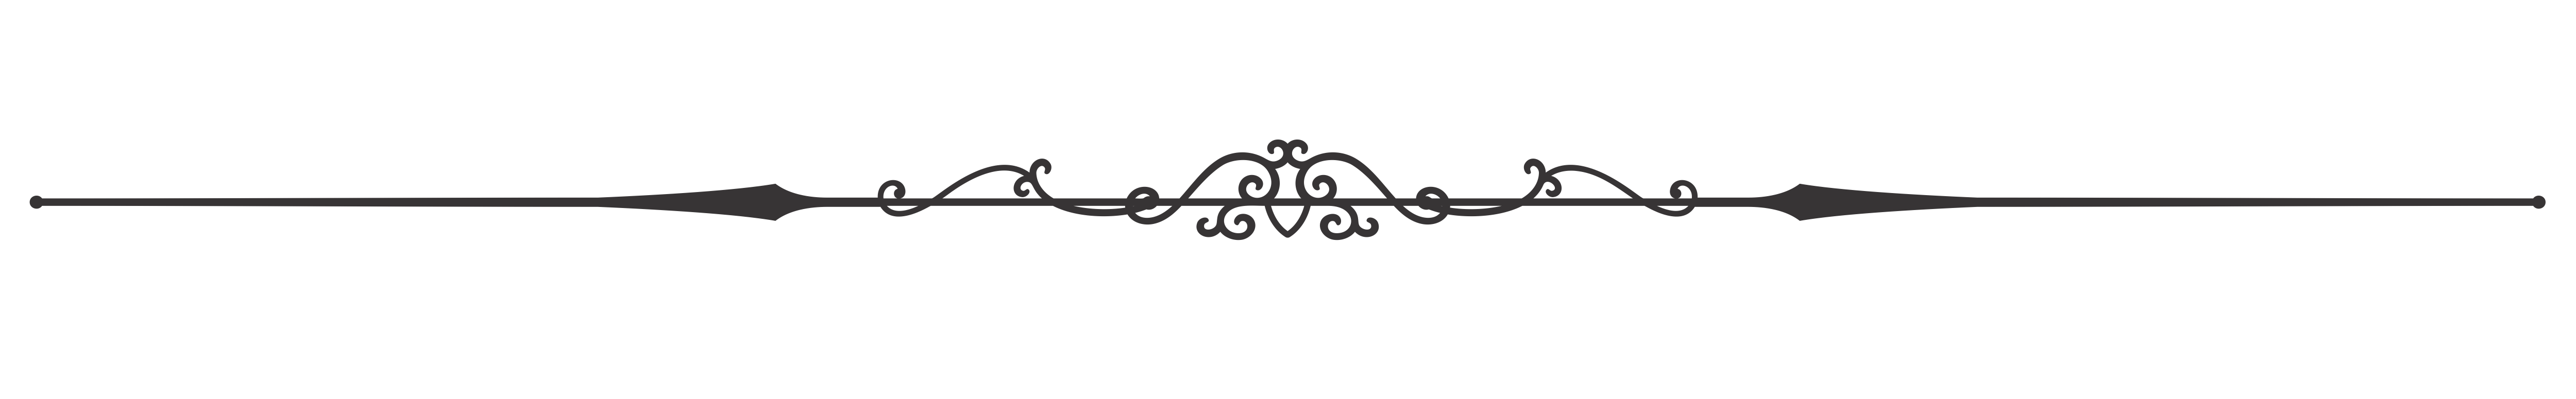
\includegraphics[width=0.8\textwidth]{line.png}
	\end{center}
 Съедена почти вся банка малинового варенья, а вот навык 'делать заранее' и 'решать проблемы сразу по мере поступления', к сожалению, нет :с

